\documentclass[mathserif,9pt]{beamer}
\usepackage[T1]{fontenc}
\usepackage[utf8]{inputenc}
\usepackage[ngerman]{babel}        % German style for date, sections ...

%\usepackage{helvet}

% Teilweise nützeliche Pakete:
%\usepackage[USenglish,english,ngerman]{babel}
%\usepackage{fancyhdr}
%\usepackage{hyperref}
%\usepackage{graphicx}
%\usepackage{array}
\usepackage{tikz}
\usepackage{verbatim}
\usetikzlibrary{arrows,automata}
%\usepackage{fancyvrb}
%\usepackage{ctable}
%\usepackage{longtable}
%\usepackage{hhline}
%\usepackage{varioref}
%\usepackage{wrapfig}
%\usepackage{subfigure}
%\usepackage{eurosym}
%\usepackage{lmodern}
%\usepackage{hvfloat}
\usepackage{tabularx}
%\usepackage{bibgerm}
%\usepackage{listings}
%\usepackage{color}
% \usepackage{tocloft} Errors!

\usepackage{fbtechnik-slides-100917}
\usepackage{graphicx}    % custom beamer style file: HS Emden/Leer

\title[Einarmiger Arduit]{Einarmiger Arduit}
\subtitle{Glücksspiel kann Süchtig machen}
\author{Arbeitstechniken Gruppe 64}
\institute{Franziska Massmann \; Jonas Nikolić \; Lukas Pensler \; Simon Struck}
\date{\today}

%\date[31. August 2010]{\vspace{-30pt}\\31. August 2010\\[10pt]
%{\scriptsize
%\begin{tabular}{ll}
%	Erstprüfer:	& Prof. Dr. ... \\
%	Zweitprüfer:& Prof. Dr. ... \\
%\end{tabular}\\[-0cm]}}

\begin{document}
    \titleframe        % custom title frame with background logo

    \begin{frame}{Inhalt}
        %\begin{eblock}
        %\vspace{-1em}
        \tableofcontents{}
        %[hideallsubsections]
        %\end{eblock}
    \end{frame}

    \section{Wortschöpfung}
    \begin{frame}{}
        %			\framesubtitle{NANANA}
        \begin{block}{}
            \centering
            \Huge{
            Einarmiger Bandit \\
            + \\
            Arduino \\
            = \\
            Einarmiger Arduit}
        \end{block}
    \end{frame}

    \section{Unser Ziel}
    \begin{frame}{Unser Ziel}
        \begin{block}{Einarmiger Bandit mit einem Arduino und 7-Segment Displays}
            \begin{itemize}
                \item Spielekonsole nicht umsetzbar (zu teuer)
                \item Echte Rollen zu teuer und zu komplex
                \item LCD\,--\,Bildschirm nicht interessant genug
            \end{itemize}
        \end{block}
    \end{frame}

    \section{Umsetzung}
    \subsection{Schaltung}
    \begin{frame}{Schaltung}
        \begin{block}{}
            \begin{minipage}[c]{0.6\textwidth}
                \begin{itemize}
                    \item 7-Segment-Displays simulieren Rollen
                    \item Schieberegister in daisychain für genug Ausgänge
                    \item Taster an interupt-Pin 
                \end{itemize}
            \end{minipage}
            \hfill
            \begin{minipage}[c]{0.3\textwidth}
               \begin{figure} 
                    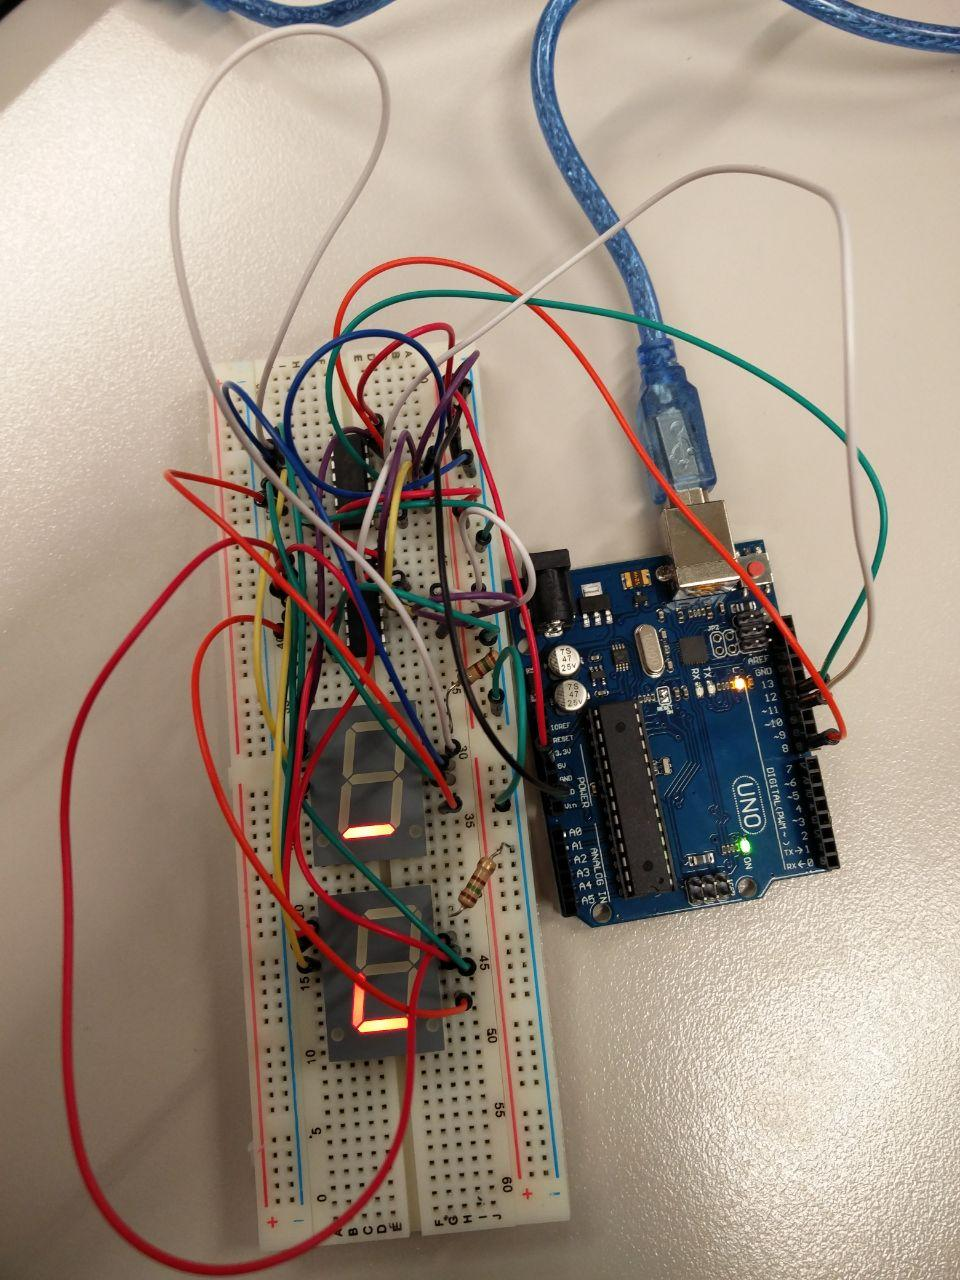
\includegraphics[width=\textwidth]{img/breadboard.jpg}
                    \caption{erster Test d. Segmentanzeigen}
                    \label{fig:breadboard}
               \end{figure}
            \end{minipage}
        \end{block}
    \end{frame}

    \begin{frame}{Schaltung}
        \begin{block}{Displays und Schieberegister}
            \begin{minipage}[c]{0.6\textwidth}
                \begin{itemize}
                    \item 
                \end{itemize}
            \end{minipage}
            \hfill
            \begin{minipage}[c]{0.3\textwidth}
               \begin{figure} 
                    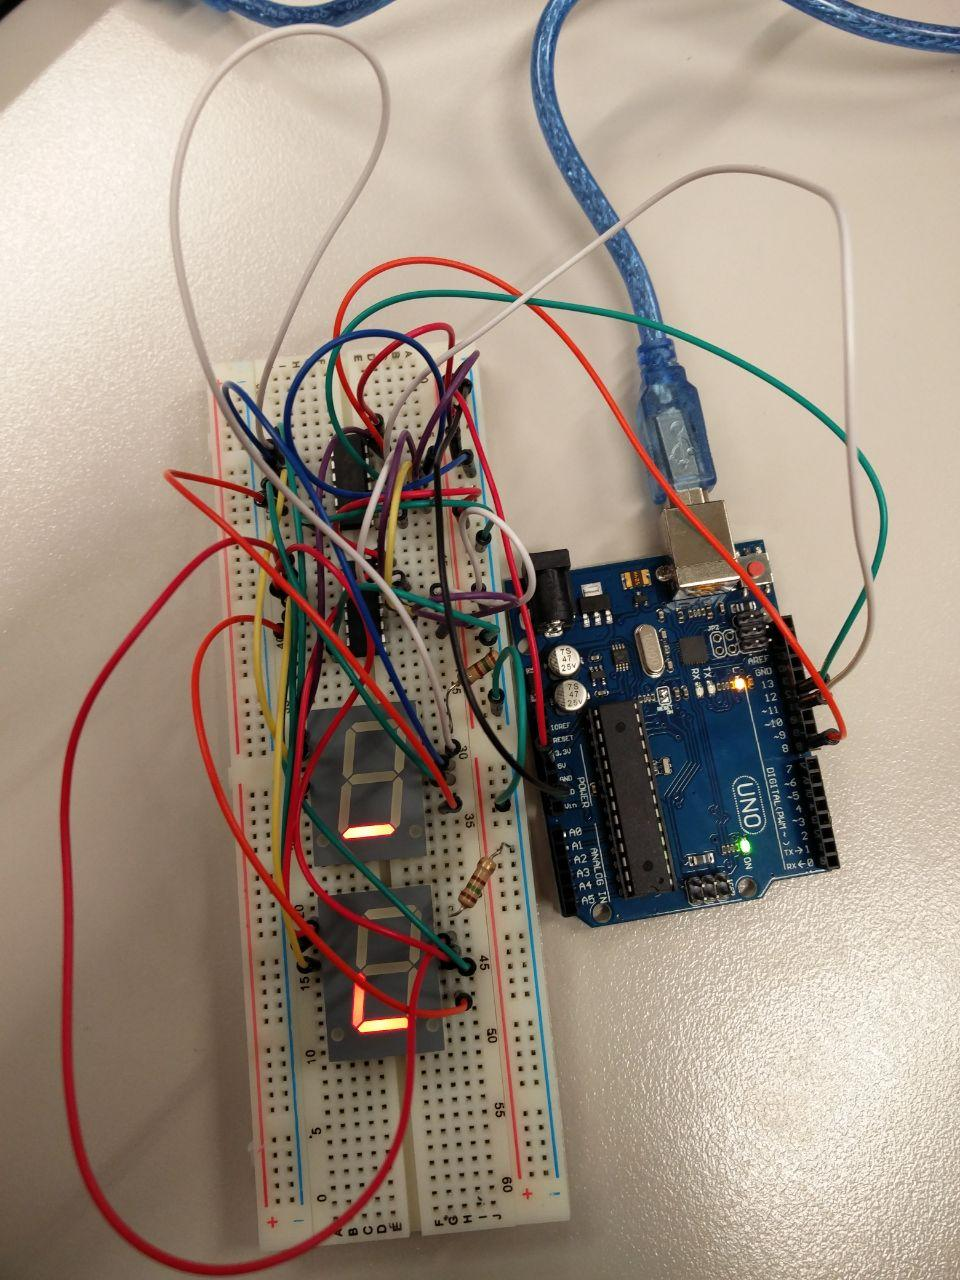
\includegraphics[width=\textwidth]{img/breadboard.jpg}
                    \caption{erster Test d. Segmentanzeigen}
                    \label{fig:breadboard}
               \end{figure}
            \end{minipage}
        \end{block}
    \end{frame}

    \subsection{Code}
    \begin{frame}{Code}
        \begin{block}{}
            \begin{itemize}
                \item State Machine --- Kontrolliert animationen
                \item Interrupt --- Verarbeitet Input nur wenn welcher da ist
                \item Animationen --- Durch Algorithmus generiert um Platz zu sparen
            \end{itemize}
        \end{block}
    \end{frame}
    
    \subsubsection*{State Machine}
    \begin{frame}{State Machine}
        \begin{block}{}
            \begin{figure}
                \centering
                 \begin{tikzpicture}[->, >=stealth', shorten >=1pt, auto, node distance=3cm, font=\footnotesize]
                
                      \node[initial,state]    (off)               {Off};
                      \node[state]            (z0) [right of=off, node distance=2cm] {Idle};
                      \node[state]            (z1) [right of=z0] {Spin up};
                      \node[state]            (z2) [below right of=z1] {Spinning};
                      \node[state]            (z3) [below left of=z2] {Spin down};
                      \node[state]            (z4) [left of=z3] {Show Result};
                    
                      \path (off) edge node        {} (z0)
                            (z0) edge node        {Hebel ziehen}   (z1)
                            (z1) edge node        {$\Delta t$} (z2)
                            (z2) edge node        {$\Delta t$} (z3)
                            (z3) edge node [swap] {$\Delta t$} (z4)
                            (z4) edge node        {$\Delta t$} (z0)
                            (z4) edge node [swap] {Hebel ziehen} (z1);
                \end{tikzpicture}
                \caption{Interne StateMachine des Automaten}
                \label{gra:statemachine}
            \end{figure}
        \end{block}
    \end{frame}

    \subsection{Gehäuse}
    \begin{frame}{Gehäuse}
        \begin{block}{}
            \begin{itemize}
                \item Stabiles und leichtes Material
                \item Ergonomischer Bau
                \item Auf dem Tisch platziert sollen Rollen auf Augenhöhe sein
            \end{itemize}
            \begin{figure}
                \centering
                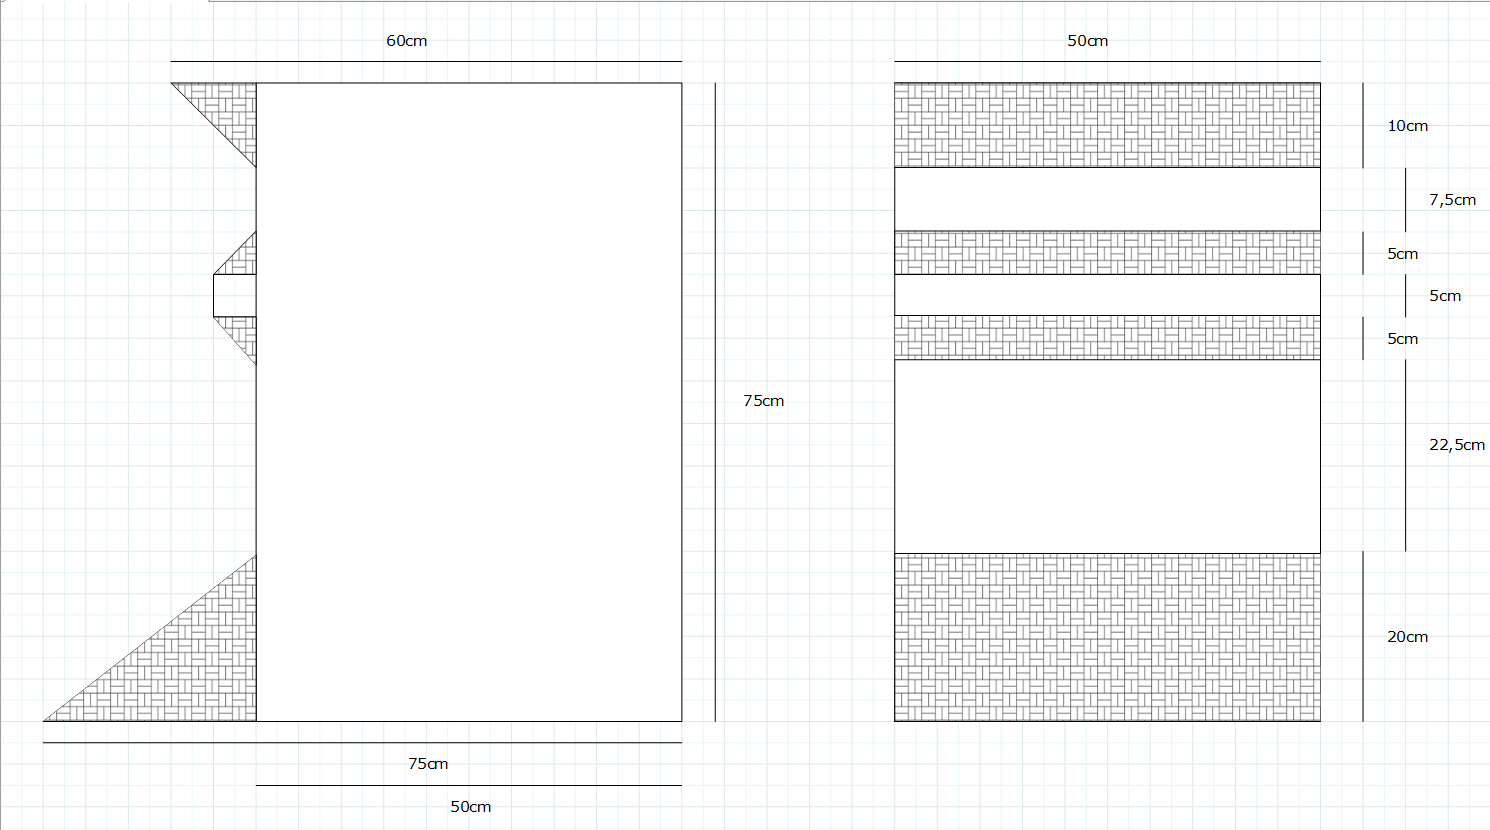
\includegraphics[height=0.4\paperheight]{img/gehause.png}
                \caption{Erste Version des Geh\"auses}
                \label{fig:gehausev1}
            \end{figure}
        \end{block}
    \end{frame}
    
    \begin{frame}{Gehäuse}
        \begin{block}{Version 2}
            \begin{figure}
                \centering
                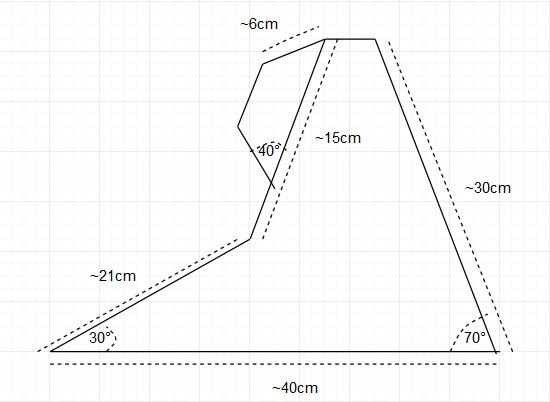
\includegraphics[height=0.5\paperheight]{img/gehause-version2.jpeg}
                \caption{Zweite Version des Geh\"auses}
                \label{fig:gehausev2}
            \end{figure}
        \end{block}
    \end{frame}

    \subsection{Software}
    \begin{frame}{Software}
        \begin{block}{}
            \begin{tabular}{cll}
                
\includegraphics[width=3.5mm]{img/drawio.png} & Draw.io & Diagramme erstellen \\
                
\includegraphics[width=3.5mm]{img/fritzing.png} & Fritzing & Schaltung Design \\
                
\includegraphics[width=3.5mm]{img/github.png} & Github & Quellcode teilen \\
                
\includegraphics[width=3.5mm]{img/googledrive.png} & Google Drive & Dokumente teilen \\
                
\includegraphics[width=3.5mm]{img/platformio.png} & PlatformIO (Atom) & Quellcode editieren \\
                
\includegraphics[width=3.5mm]{img/trello.png} & Trello & Organisieren \\
            \end{tabular}
        \end{block}
    \end{frame}
    \section{Demonstration}
    \begin{frame}
        \begin{block}{}
            \centering
						{\fontsize{51.59}{51.59}\selectfont Demo}
        \end{block}
    \end{frame}

    \section{Fazit}
    \begin{frame}
        \begin{block}{Aktueller Fortschritt:}
            \begin{itemize}{}
                \item Code: In Arbeit
                \item Gehäuse: Geplant
                \item Schaltung: Prototyp im Bau
            \end{itemize}
        \end{block}
    \end{frame}

    %\section{Abbildungsverzeichnis}
    %\begin{frame}{Abbildungsverzeichnis}
    %    \begin{block}{}
    %    \listoffigures{}
    %    \end{block}
    %\end{frame}
    
    \begin{frame}{Ende}
        \begin{block}{Ende}
            Vielen Dank für Ihre Aufmerksamkeit \ldots
        \end{block}
    \end{frame}

    \begin{frame}{Literatur}
    	\footnotesize
    	\nocite*
      \bibliography{literatur}
    	\bibliographystyle{geralpha}
    \end{frame}

\end{document}
